% Options for packages loaded elsewhere
\PassOptionsToPackage{unicode}{hyperref}
\PassOptionsToPackage{hyphens}{url}
%
\documentclass[
]{article}
\usepackage{amsmath,amssymb}
\usepackage{lmodern}
\usepackage{iftex}
\ifPDFTeX
  \usepackage[T1]{fontenc}
  \usepackage[utf8]{inputenc}
  \usepackage{textcomp} % provide euro and other symbols
\else % if luatex or xetex
  \usepackage{unicode-math}
  \defaultfontfeatures{Scale=MatchLowercase}
  \defaultfontfeatures[\rmfamily]{Ligatures=TeX,Scale=1}
\fi
% Use upquote if available, for straight quotes in verbatim environments
\IfFileExists{upquote.sty}{\usepackage{upquote}}{}
\IfFileExists{microtype.sty}{% use microtype if available
  \usepackage[]{microtype}
  \UseMicrotypeSet[protrusion]{basicmath} % disable protrusion for tt fonts
}{}
\makeatletter
\@ifundefined{KOMAClassName}{% if non-KOMA class
  \IfFileExists{parskip.sty}{%
    \usepackage{parskip}
  }{% else
    \setlength{\parindent}{0pt}
    \setlength{\parskip}{6pt plus 2pt minus 1pt}}
}{% if KOMA class
  \KOMAoptions{parskip=half}}
\makeatother
\usepackage{xcolor}
\usepackage[margin=1in]{geometry}
\usepackage{color}
\usepackage{fancyvrb}
\newcommand{\VerbBar}{|}
\newcommand{\VERB}{\Verb[commandchars=\\\{\}]}
\DefineVerbatimEnvironment{Highlighting}{Verbatim}{commandchars=\\\{\}}
% Add ',fontsize=\small' for more characters per line
\usepackage{framed}
\definecolor{shadecolor}{RGB}{248,248,248}
\newenvironment{Shaded}{\begin{snugshade}}{\end{snugshade}}
\newcommand{\AlertTok}[1]{\textcolor[rgb]{0.94,0.16,0.16}{#1}}
\newcommand{\AnnotationTok}[1]{\textcolor[rgb]{0.56,0.35,0.01}{\textbf{\textit{#1}}}}
\newcommand{\AttributeTok}[1]{\textcolor[rgb]{0.77,0.63,0.00}{#1}}
\newcommand{\BaseNTok}[1]{\textcolor[rgb]{0.00,0.00,0.81}{#1}}
\newcommand{\BuiltInTok}[1]{#1}
\newcommand{\CharTok}[1]{\textcolor[rgb]{0.31,0.60,0.02}{#1}}
\newcommand{\CommentTok}[1]{\textcolor[rgb]{0.56,0.35,0.01}{\textit{#1}}}
\newcommand{\CommentVarTok}[1]{\textcolor[rgb]{0.56,0.35,0.01}{\textbf{\textit{#1}}}}
\newcommand{\ConstantTok}[1]{\textcolor[rgb]{0.00,0.00,0.00}{#1}}
\newcommand{\ControlFlowTok}[1]{\textcolor[rgb]{0.13,0.29,0.53}{\textbf{#1}}}
\newcommand{\DataTypeTok}[1]{\textcolor[rgb]{0.13,0.29,0.53}{#1}}
\newcommand{\DecValTok}[1]{\textcolor[rgb]{0.00,0.00,0.81}{#1}}
\newcommand{\DocumentationTok}[1]{\textcolor[rgb]{0.56,0.35,0.01}{\textbf{\textit{#1}}}}
\newcommand{\ErrorTok}[1]{\textcolor[rgb]{0.64,0.00,0.00}{\textbf{#1}}}
\newcommand{\ExtensionTok}[1]{#1}
\newcommand{\FloatTok}[1]{\textcolor[rgb]{0.00,0.00,0.81}{#1}}
\newcommand{\FunctionTok}[1]{\textcolor[rgb]{0.00,0.00,0.00}{#1}}
\newcommand{\ImportTok}[1]{#1}
\newcommand{\InformationTok}[1]{\textcolor[rgb]{0.56,0.35,0.01}{\textbf{\textit{#1}}}}
\newcommand{\KeywordTok}[1]{\textcolor[rgb]{0.13,0.29,0.53}{\textbf{#1}}}
\newcommand{\NormalTok}[1]{#1}
\newcommand{\OperatorTok}[1]{\textcolor[rgb]{0.81,0.36,0.00}{\textbf{#1}}}
\newcommand{\OtherTok}[1]{\textcolor[rgb]{0.56,0.35,0.01}{#1}}
\newcommand{\PreprocessorTok}[1]{\textcolor[rgb]{0.56,0.35,0.01}{\textit{#1}}}
\newcommand{\RegionMarkerTok}[1]{#1}
\newcommand{\SpecialCharTok}[1]{\textcolor[rgb]{0.00,0.00,0.00}{#1}}
\newcommand{\SpecialStringTok}[1]{\textcolor[rgb]{0.31,0.60,0.02}{#1}}
\newcommand{\StringTok}[1]{\textcolor[rgb]{0.31,0.60,0.02}{#1}}
\newcommand{\VariableTok}[1]{\textcolor[rgb]{0.00,0.00,0.00}{#1}}
\newcommand{\VerbatimStringTok}[1]{\textcolor[rgb]{0.31,0.60,0.02}{#1}}
\newcommand{\WarningTok}[1]{\textcolor[rgb]{0.56,0.35,0.01}{\textbf{\textit{#1}}}}
\usepackage{graphicx}
\makeatletter
\def\maxwidth{\ifdim\Gin@nat@width>\linewidth\linewidth\else\Gin@nat@width\fi}
\def\maxheight{\ifdim\Gin@nat@height>\textheight\textheight\else\Gin@nat@height\fi}
\makeatother
% Scale images if necessary, so that they will not overflow the page
% margins by default, and it is still possible to overwrite the defaults
% using explicit options in \includegraphics[width, height, ...]{}
\setkeys{Gin}{width=\maxwidth,height=\maxheight,keepaspectratio}
% Set default figure placement to htbp
\makeatletter
\def\fps@figure{htbp}
\makeatother
\setlength{\emergencystretch}{3em} % prevent overfull lines
\providecommand{\tightlist}{%
  \setlength{\itemsep}{0pt}\setlength{\parskip}{0pt}}
\setcounter{secnumdepth}{-\maxdimen} % remove section numbering
\ifLuaTeX
  \usepackage{selnolig}  % disable illegal ligatures
\fi
\IfFileExists{bookmark.sty}{\usepackage{bookmark}}{\usepackage{hyperref}}
\IfFileExists{xurl.sty}{\usepackage{xurl}}{} % add URL line breaks if available
\urlstyle{same} % disable monospaced font for URLs
\hypersetup{
  pdftitle={Comments on Gini Map of Vietnam},
  pdfauthor={Hiroshi Suzuki},
  hidelinks,
  pdfcreator={LaTeX via pandoc}}

\title{Comments on Gini Map of Vietnam}
\author{Hiroshi Suzuki}
\date{}

\begin{document}
\maketitle

\hypertarget{setup}{%
\section{Setup}\label{setup}}

I tried to use a smallest set of packages to understand the
functionality of each package clearly.

\begin{Shaded}
\begin{Highlighting}[]
\FunctionTok{library}\NormalTok{(tidyverse)}
\end{Highlighting}
\end{Shaded}

\begin{verbatim}
## -- Attaching core tidyverse packages ------------------------ tidyverse 2.0.0 --
## v dplyr     1.1.1     v readr     2.1.4
## v forcats   1.0.0     v stringr   1.5.0
## v ggplot2   3.4.2     v tibble    3.2.1
## v lubridate 1.9.2     v tidyr     1.3.0
## v purrr     1.0.1     
## -- Conflicts ------------------------------------------ tidyverse_conflicts() --
## x dplyr::filter() masks stats::filter()
## x dplyr::lag()    masks stats::lag()
## i Use the conflicted package (<http://conflicted.r-lib.org/>) to force all conflicts to become errors
\end{verbatim}

\begin{Shaded}
\begin{Highlighting}[]
\FunctionTok{library}\NormalTok{(readxl)}
\FunctionTok{library}\NormalTok{(maps)}
\end{Highlighting}
\end{Shaded}

\begin{verbatim}
## 
## Attaching package: 'maps'
## 
## The following object is masked from 'package:purrr':
## 
##     map
\end{verbatim}

\begin{Shaded}
\begin{Highlighting}[]
\FunctionTok{library}\NormalTok{(sf)}
\end{Highlighting}
\end{Shaded}

\begin{verbatim}
## Linking to GEOS 3.11.0, GDAL 3.5.3, PROJ 9.1.0; sf_use_s2() is TRUE
\end{verbatim}

\hypertarget{gini-data}{%
\subsection{Gini Data}\label{gini-data}}

\hypertarget{import-gini-of-the-world-data}{%
\subsection{Import GINI of the World
Data}\label{import-gini-of-the-world-data}}

The following is my personal memo:

\begin{quote}
Gini index Gini index measures the extent to which the distribution of
income (or, in some cases, consumption expenditure) among individuals or
households within an economy deviates from a perfectly equal
distribution. A Lorenz curve plots the cumulative percentages of total
income received against the cumulative number of recipients, starting
with the poorest individual or household. The Gini index measures the
area between the Lorenz curve and a hypothetical line of absolute
equality, expressed as a percentage of the maximum area under the line.
Thus a Gini index of 0 represents perfect equality, while an index of
100 implies perfect inequality.
\url{https://data.worldbank.org/indicator/SI.POV.GINI}
\end{quote}

\begin{Shaded}
\begin{Highlighting}[]
\NormalTok{gini\_world }\OtherTok{\textless{}{-}} \FunctionTok{read\_excel}\NormalTok{(}\StringTok{\textquotesingle{}Giniworld.xlsx\textquotesingle{}}\NormalTok{)}
\NormalTok{gini\_world}
\end{Highlighting}
\end{Shaded}

\begin{verbatim}
## # A tibble: 269 x 2
##    country                       Gini
##    <chr>                        <dbl>
##  1 Aruba                       NA    
##  2 Africa Eastern and Southern NA    
##  3 Afghanistan                 NA    
##  4 Africa Western and Central  NA    
##  5 Angola                       0.513
##  6 Albania                      0.294
##  7 Andorra                     NA    
##  8 Arab World                  NA    
##  9 United Arab Emirates         0.26 
## 10 Argentina                    0.42 
## # i 259 more rows
\end{verbatim}

\hypertarget{world-map}{%
\subsection{World Map}\label{world-map}}

See class note.

\begin{Shaded}
\begin{Highlighting}[]
\NormalTok{world\_map }\OtherTok{\textless{}{-}} \FunctionTok{map\_data}\NormalTok{(}\StringTok{"world"}\NormalTok{)}
\NormalTok{world\_map\_rev }\OtherTok{\textless{}{-}}\NormalTok{ world\_map }\SpecialCharTok{\%\textgreater{}\%} 
  \FunctionTok{mutate}\NormalTok{(}\AttributeTok{region =} \FunctionTok{case\_when}\NormalTok{(region }\SpecialCharTok{==} \StringTok{"Macedonia"} \SpecialCharTok{\textasciitilde{}} \StringTok{"North Macedonia"}\NormalTok{,}
\NormalTok{                            region }\SpecialCharTok{==} \StringTok{"Ivory Coast"}  \SpecialCharTok{\textasciitilde{}} \StringTok{"Cote d\textquotesingle{}Ivoire"}\NormalTok{,}
\NormalTok{                            region }\SpecialCharTok{==} \StringTok{"Democratic Republic of the Congo"}  \SpecialCharTok{\textasciitilde{}} \StringTok{"Congo, Dem. Rep."}\NormalTok{,}
\NormalTok{                            region }\SpecialCharTok{==} \StringTok{"Republic of Congo"} \SpecialCharTok{\textasciitilde{}}  \StringTok{"Congo, Rep."}\NormalTok{,}
\NormalTok{                            region }\SpecialCharTok{==} \StringTok{"UK"} \SpecialCharTok{\textasciitilde{}}  \StringTok{"United Kingdom"}\NormalTok{,}
\CommentTok{\#                            region == "USA" \textasciitilde{}  "United States",}
\NormalTok{                            region }\SpecialCharTok{==} \StringTok{"Laos"} \SpecialCharTok{\textasciitilde{}}  \StringTok{"Lao PDR"}\NormalTok{,}
\NormalTok{                            region }\SpecialCharTok{==} \StringTok{"Slovakia"} \SpecialCharTok{\textasciitilde{}}  \StringTok{"Slovak Republic"}\NormalTok{,}
\NormalTok{                            region }\SpecialCharTok{==} \StringTok{"Saint Lucia"} \SpecialCharTok{\textasciitilde{}}  \StringTok{"St. Lucia"}\NormalTok{,}
\NormalTok{                            region }\SpecialCharTok{==} \StringTok{"Kyrgyzstan"}  \SpecialCharTok{\textasciitilde{}}  \StringTok{"Kyrgyz Republic"}\NormalTok{,}
\NormalTok{                            region }\SpecialCharTok{==} \StringTok{"Micronesia"} \SpecialCharTok{\textasciitilde{}} \StringTok{"Micronesia, Fed. Sts."}\NormalTok{,}
\NormalTok{                            region }\SpecialCharTok{==} \StringTok{"Swaziland"}  \SpecialCharTok{\textasciitilde{}} \StringTok{"Eswatini"}\NormalTok{, }
\NormalTok{                            region }\SpecialCharTok{==} \StringTok{"Virgin Islands"}  \SpecialCharTok{\textasciitilde{}} \StringTok{"Virgin Islands (U.S.)"}\NormalTok{, }
\CommentTok{\#                            region == "Russia" \textasciitilde{} "Russian Federation", }
\NormalTok{                            region }\SpecialCharTok{==} \StringTok{"Egypt"} \SpecialCharTok{\textasciitilde{}} \StringTok{"Egypt, Arab Rep."}\NormalTok{,}
\NormalTok{                            region }\SpecialCharTok{==} \StringTok{"South Korea"} \SpecialCharTok{\textasciitilde{}} \StringTok{"Korea, Rep."}\NormalTok{,}
\NormalTok{                            region }\SpecialCharTok{==} \StringTok{"North Korea"} \SpecialCharTok{\textasciitilde{}} \StringTok{"Korea, Dem. People\textquotesingle{}s Rep."}\NormalTok{,}
\NormalTok{                            region }\SpecialCharTok{==} \StringTok{"Iran"} \SpecialCharTok{\textasciitilde{}} \StringTok{"Iran, Islamic Rep."}\NormalTok{,}
\NormalTok{                            region }\SpecialCharTok{==} \StringTok{"Brunei"} \SpecialCharTok{\textasciitilde{}} \StringTok{"Brunei Darussalam"}\NormalTok{,}
\NormalTok{                            region }\SpecialCharTok{==} \StringTok{"Venezuela"} \SpecialCharTok{\textasciitilde{}} \StringTok{"Venezuela, RB"}\NormalTok{,}
\NormalTok{                            region }\SpecialCharTok{==} \StringTok{"Yemen"} \SpecialCharTok{\textasciitilde{}} \StringTok{"Yemen, Rep."}\NormalTok{,}
\NormalTok{                            region }\SpecialCharTok{==} \StringTok{"Bahamas"} \SpecialCharTok{\textasciitilde{}} \StringTok{"Bahamas, The"}\NormalTok{,}
\NormalTok{                            region }\SpecialCharTok{==} \StringTok{"Syria"} \SpecialCharTok{\textasciitilde{}} \StringTok{"Syrian Arab Republic"}\NormalTok{,}
\NormalTok{                            region }\SpecialCharTok{==} \StringTok{"Turkey"} \SpecialCharTok{\textasciitilde{}} \StringTok{"Turkiye"}\NormalTok{,}
\NormalTok{                            region }\SpecialCharTok{==} \StringTok{"Cape Verde"} \SpecialCharTok{\textasciitilde{}} \StringTok{"Cabo Verde"}\NormalTok{,}
\NormalTok{                            region }\SpecialCharTok{==} \StringTok{"Gambia"} \SpecialCharTok{\textasciitilde{}} \StringTok{"Gambia, The"}\NormalTok{,}
\NormalTok{                            region }\SpecialCharTok{==} \StringTok{"Czech Republic"} \SpecialCharTok{\textasciitilde{}} \StringTok{"Czechia"}\NormalTok{,}
                            \ConstantTok{TRUE} \SpecialCharTok{\textasciitilde{}}\NormalTok{ region))}
\end{Highlighting}
\end{Shaded}

\hypertarget{import-gini-of-viet-nam-data}{%
\subsection{Import Gini of Viet Nam
Data}\label{import-gini-of-viet-nam-data}}

Used your data.

\begin{Shaded}
\begin{Highlighting}[]
\NormalTok{gini\_vietnam }\OtherTok{\textless{}{-}} \FunctionTok{read\_excel}\NormalTok{(}\StringTok{\textquotesingle{}DataVN.xls\textquotesingle{}}\NormalTok{)}
\NormalTok{gini\_vietnam}
\end{Highlighting}
\end{Shaded}

\begin{verbatim}
## # A tibble: 63 x 16
##       id province   `sub region`     gini icgap top20 `GDP 2021 (Billion VND)`
##    <dbl> <chr>      <chr>           <dbl> <dbl> <dbl>                    <dbl>
##  1     1 Ha Noi     Red River Delta 0.338  6.32  42.1                 1067540 
##  2     2 Vinh Phuc  Red River Delta 0.284  4.78  39.5                  136183 
##  3     3 Bac Ninh   Red River Delta 0.288  4.98  39.0                  227615.
##  4     4 Quang Ninh Red River Delta 0.260  4.30  36.5                  238186.
##  5     5 Hai Duong  Red River Delta 0.295  5.21  41.0                  149090 
##  6     6 Hai Phong  Red River Delta 0.264  4.24  37.7                  315710.
##  7     7 Hung Yen   Red River Delta 0.264  4.68  36.2                  112306.
##  8     8 Thai Binh  Red River Delta 0.207  3.25  32.5                   98310 
##  9     9 Ha Nam     Red River Delta 0.297  5.55  39.6                   66895.
## 10    10 Nam Dinh   Red River Delta 0.190  2.93  32.1                   84097.
## # i 53 more rows
## # i 9 more variables: `GDPPC (Thoudsand VND)` <dbl>, Investment <dbl>,
## #   emp <dbl>, lit <dbl>, edu <dbl>, pop <dbl>, poprate <dbl>, ubrate <dbl>,
## #   `General average income` <dbl>
\end{verbatim}

\begin{Shaded}
\begin{Highlighting}[]
\FunctionTok{colnames}\NormalTok{(gini\_vietnam)}
\end{Highlighting}
\end{Shaded}

\begin{verbatim}
##  [1] "id"                     "province"               "sub region"            
##  [4] "gini"                   "icgap"                  "top20"                 
##  [7] "GDP 2021 (Billion VND)" "GDPPC (Thoudsand VND)"  "Investment"            
## [10] "emp"                    "lit"                    "edu"                   
## [13] "pop"                    "poprate"                "ubrate"                
## [16] "General average income"
\end{verbatim}

\hypertarget{gini-map-of-the-world}{%
\section{Gini Map of the World}\label{gini-map-of-the-world}}

\begin{Shaded}
\begin{Highlighting}[]
\NormalTok{gini\_world }\SpecialCharTok{\%\textgreater{}\%} \FunctionTok{arrange}\NormalTok{(country)}
\end{Highlighting}
\end{Shaded}

\begin{verbatim}
## # A tibble: 269 x 2
##    country                       Gini
##    <chr>                        <dbl>
##  1 Afghanistan                 NA    
##  2 Africa Eastern and Southern NA    
##  3 Africa Western and Central  NA    
##  4 Albania                      0.294
##  5 Algeria                      0.276
##  6 American Samoa              NA    
##  7 Andorra                     NA    
##  8 Angola                       0.513
##  9 Antigua and Barbuda         NA    
## 10 Arab World                  NA    
## # i 259 more rows
\end{verbatim}

\begin{Shaded}
\begin{Highlighting}[]
\NormalTok{world\_map\_rev }\SpecialCharTok{\%\textgreater{}\%} \FunctionTok{distinct}\NormalTok{(region) }\SpecialCharTok{\%\textgreater{}\%} 
  \FunctionTok{anti\_join}\NormalTok{(gini\_world, }\AttributeTok{by =} \FunctionTok{c}\NormalTok{(}\StringTok{"region"} \OtherTok{=} \StringTok{"country"}\NormalTok{)) }\SpecialCharTok{\%\textgreater{}\%} \FunctionTok{as\_tibble}\NormalTok{()}
\end{Highlighting}
\end{Shaded}

\begin{verbatim}
## # A tibble: 50 x 1
##    region                             
##    <chr>                              
##  1 Anguilla                           
##  2 Antarctica                         
##  3 French Southern and Antarctic Lands
##  4 Antigua                            
##  5 Barbuda                            
##  6 Saint Barthelemy                   
##  7 Cook Islands                       
##  8 Canary Islands                     
##  9 Falkland Islands                   
## 10 Reunion                            
## # i 40 more rows
\end{verbatim}

\begin{itemize}
\tightlist
\item
  There are many missing countries in world map. If you use it please
  check carefully.
\end{itemize}

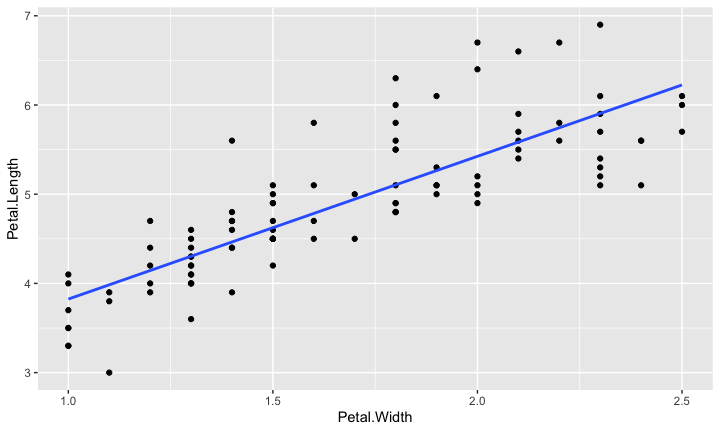
\includegraphics{le-map_revised_files/figure-latex/unnamed-chunk-8-1.pdf}

\hypertarget{gini-map-of-vietnam-part-i}{%
\section{Gini Map of Vietnam, Part I}\label{gini-map-of-vietnam-part-i}}

I used a different map data (in spatial format) of Vietnam in the
following.

Source: \url{https://rpubs.com/Linh-LTP/890658}

\begin{Shaded}
\begin{Highlighting}[]
\NormalTok{link }\OtherTok{\textless{}{-}} \StringTok{"https://data.opendevelopmentmekong.net/dataset/999c96d8{-}fae0{-}4b82{-}9a2b{-}e481f6f50e12/resource/2818c2c5{-}e9c3{-}440b{-}a9b8{-}3029d7298065/download/diaphantinhenglish.geojson?fbclid=IwAR1coUVLkuEoJRsgaH81q6ocz1nVeGBirqpKRBN8WWxXQIJREUL1buFi1eE"}

\NormalTok{vn\_spatial }\OtherTok{\textless{}{-}} \FunctionTok{st\_read}\NormalTok{(link)}
\end{Highlighting}
\end{Shaded}

\begin{verbatim}
## Reading layer `OGRGeoJSON' from data source 
##   `https://data.opendevelopmentmekong.net/dataset/999c96d8-fae0-4b82-9a2b-e481f6f50e12/resource/2818c2c5-e9c3-440b-a9b8-3029d7298065/download/diaphantinhenglish.geojson?fbclid=IwAR1coUVLkuEoJRsgaH81q6ocz1nVeGBirqpKRBN8WWxXQIJREUL1buFi1eE' 
##   using driver `GeoJSON'
## Simple feature collection with 63 features and 2 fields
## Geometry type: MULTIPOLYGON
## Dimension:     XY
## Bounding box:  xmin: 102.1421 ymin: 6.953306 xmax: 116.9473 ymax: 23.3939
## Geodetic CRS:  WGS 84
\end{verbatim}

\hypertarget{test}{%
\subsection{Test}\label{test}}

\begin{Shaded}
\begin{Highlighting}[]
\FunctionTok{ggplot}\NormalTok{() }\SpecialCharTok{+} 
  \FunctionTok{geom\_sf}\NormalTok{(}\AttributeTok{data =}\NormalTok{ vn\_spatial) }\SpecialCharTok{+} 
  \FunctionTok{labs}\NormalTok{(}\AttributeTok{title =} \StringTok{"Vietnam Map {-} Provinces"}\NormalTok{)}
\end{Highlighting}
\end{Shaded}

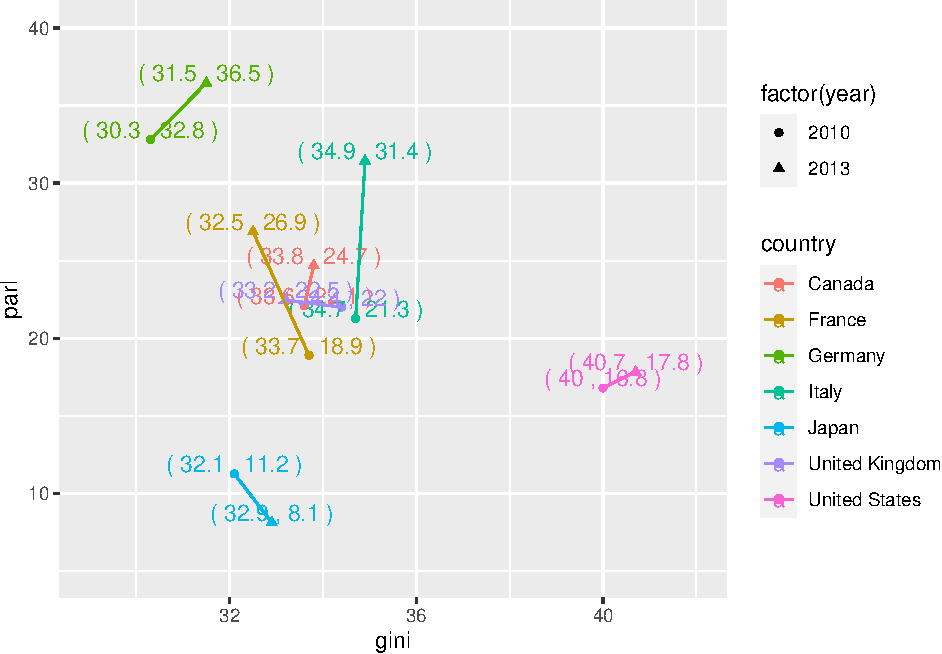
\includegraphics{le-map_revised_files/figure-latex/unnamed-chunk-10-1.pdf}

\hypertarget{compare-with-gini-data-of-vietnam}{%
\subsection{Compare with Gini Data of
Vietnam}\label{compare-with-gini-data-of-vietnam}}

\begin{Shaded}
\begin{Highlighting}[]
\NormalTok{vn\_spatial }\SpecialCharTok{\%\textgreater{}\%} \FunctionTok{as\_tibble}\NormalTok{() }\SpecialCharTok{\%\textgreater{}\%} \FunctionTok{arrange}\NormalTok{(Name)}
\end{Highlighting}
\end{Shaded}

\begin{verbatim}
## # A tibble: 63 x 3
##    Code  Name                                                           geometry
##    <chr> <chr>                                                <MULTIPOLYGON [°]>
##  1 AD01  An Giang          (((105.1152 10.95566, 105.1146 10.94692, 105.1038 10~
##  2 AD01  Ba Ria - Vung Tau (((106.0811 8.577536, 106.0807 8.577515, 106.0802 8.~
##  3 AD01  Bac Giang         (((106.1654 21.62022, 106.1692 21.6157, 106.1709 21.~
##  4 AD01  Bac Kan           (((105.7442 22.73519, 105.7462 22.73142, 105.7482 22~
##  5 AD01  Bac Lieu          (((105.3259 9.600039, 105.3275 9.599981, 105.3286 9.~
##  6 AD01  Bac Ninh          (((106.0325 21.22488, 106.0322 21.21961, 106.0322 21~
##  7 AD01  Ben Tre           (((106.4251 10.32019, 106.4447 10.30821, 106.4472 10~
##  8 AD01  Binh Dinh         (((109.3686 13.5916, 109.3682 13.59158, 109.3679 13.~
##  9 AD01  Binh Duong        (((106.4361 11.5021, 106.4433 11.50111, 106.4513 11.~
## 10 AD01  Binh Phuoc        (((107.2194 12.20223, 107.2242 12.16745, 107.2261 12~
## # i 53 more rows
\end{verbatim}

\begin{Shaded}
\begin{Highlighting}[]
\NormalTok{gini\_vietnam }\SpecialCharTok{\%\textgreater{}\%} \FunctionTok{arrange}\NormalTok{(province)}
\end{Highlighting}
\end{Shaded}

\begin{verbatim}
## # A tibble: 63 x 16
##       id province        `sub region`    gini icgap top20 GDP 2021 (Billion VN~1
##    <dbl> <chr>           <chr>          <dbl> <dbl> <dbl>                  <dbl>
##  1    57 An Giang        Mekong River ~ 0.331  6.41  42.9                 92238.
##  2    49 Ba Ria Vung Tau South East     0.353  7.02  45.3                330754.
##  3    20 Bac Giang       Northern midl~ 0.285  4.84  39.9                129837.
##  4    14 Bac Kan         Northern midl~ 0.425 11.4   50.3                 13531.
##  5    62 Bac Lieu        Mekong River ~ 0.215  3.37  33.9                 53016.
##  6     3 Bac Ninh        Red River Del~ 0.288  4.98  39.0                227615.
##  7    53 Ben Tre         Mekong River ~ 0.346  6.58  44.1                 55964.
##  8    35 Binh Dinh       North Central~ 0.352  7.84  43.3                 95311.
##  9    47 Binh Duong      South East     0.232  3.46  34.7                408860 
## 10    45 Binh Phuoc      South East     0.296  5.21  40.4                 77838.
## # i 53 more rows
## # i abbreviated name: 1: `GDP 2021 (Billion VND)`
## # i 9 more variables: `GDPPC (Thoudsand VND)` <dbl>, Investment <dbl>,
## #   emp <dbl>, lit <dbl>, edu <dbl>, pop <dbl>, poprate <dbl>, ubrate <dbl>,
## #   `General average income` <dbl>
\end{verbatim}

\begin{Shaded}
\begin{Highlighting}[]
\NormalTok{vn\_spatial }\SpecialCharTok{\%\textgreater{}\%} \FunctionTok{anti\_join}\NormalTok{(gini\_vietnam, }\AttributeTok{by =} \FunctionTok{c}\NormalTok{(}\StringTok{"Name"} \OtherTok{=} \StringTok{"province"}\NormalTok{)) }\SpecialCharTok{\%\textgreater{}\%} \FunctionTok{as\_tibble}\NormalTok{()}
\end{Highlighting}
\end{Shaded}

\begin{verbatim}
## # A tibble: 3 x 3
##   Code  Name                                                            geometry
##   <chr> <chr>                                                 <MULTIPOLYGON [°]>
## 1 AD01  Ba Ria - Vung Tau (((106.0811 8.577536, 106.0807 8.577515, 106.0802 8.5~
## 2 AD01  Thua Thien - Hue  (((107.4281 16.71097, 107.4353 16.70543, 107.4429 16.~
## 3 AD01  TP. Ho Chi Minh   (((106.9686 10.45353, 106.9674 10.45279, 106.966 10.4~
\end{verbatim}

\begin{Shaded}
\begin{Highlighting}[]
\NormalTok{vn\_spatial }\OtherTok{\textless{}{-}}\NormalTok{ vn\_spatial }\SpecialCharTok{\%\textgreater{}\%} \FunctionTok{mutate}\NormalTok{(}\AttributeTok{Name =} \FunctionTok{case\_when}\NormalTok{(}
\NormalTok{  Name }\SpecialCharTok{==} \StringTok{"Ba Ria {-} Vung Tau"} \SpecialCharTok{\textasciitilde{}} \StringTok{"Ba Ria Vung Tau"}\NormalTok{,}
\NormalTok{  Name }\SpecialCharTok{==} \StringTok{"Thua Thien {-} Hue"} \SpecialCharTok{\textasciitilde{}} \StringTok{"Thua Thien Hue"}\NormalTok{,}
\NormalTok{  Name }\SpecialCharTok{==} \StringTok{"TP. Ho Chi Minh"} \SpecialCharTok{\textasciitilde{}} \StringTok{"Ho Chi Minh City"}\NormalTok{,}
  \ConstantTok{TRUE} \SpecialCharTok{\textasciitilde{}}\NormalTok{ Name))}
\end{Highlighting}
\end{Shaded}

\hypertarget{join-two-datasets}{%
\subsection{Join Two Datasets}\label{join-two-datasets}}

\begin{Shaded}
\begin{Highlighting}[]
\NormalTok{vietnam\_gini\_map }\OtherTok{\textless{}{-}}\NormalTok{ vn\_spatial }\SpecialCharTok{\%\textgreater{}\%} \FunctionTok{left\_join}\NormalTok{(gini\_vietnam, }\AttributeTok{by =} \FunctionTok{c}\NormalTok{(}\StringTok{"Name"} \OtherTok{=} \StringTok{"province"}\NormalTok{))}
\NormalTok{vietnam\_gini\_map}
\end{Highlighting}
\end{Shaded}

\begin{verbatim}
## Simple feature collection with 63 features and 17 fields
## Geometry type: MULTIPOLYGON
## Dimension:     XY
## Bounding box:  xmin: 102.1421 ymin: 6.953306 xmax: 116.9473 ymax: 23.3939
## Geodetic CRS:  WGS 84
## First 10 features:
##    Code            Name id                              sub region    gini
## 1  AD01        An Giang 57                      Mekong River Delta 0.33112
## 2  AD01 Ba Ria Vung Tau 49                              South East 0.35304
## 3  AD01       Bac Giang 20    Northern midlands and mountain areas 0.28528
## 4  AD01         Bac Kan 14    Northern midlands and mountain areas 0.42468
## 5  AD01        Bac Lieu 62                      Mekong River Delta 0.21500
## 6  AD01        Bac Ninh  3                         Red River Delta 0.28756
## 7  AD01         Ben Tre 53                      Mekong River Delta 0.34644
## 8  AD01       Binh Dinh 35 North Central and Central coastal areas 0.35220
## 9  AD01      Binh Duong 47                              South East 0.23180
## 10 AD01      Binh Phuoc 45                              South East 0.29640
##        icgap    top20 GDP 2021 (Billion VND) GDPPC (Thoudsand VND) Investment
## 1   6.411043 42.89568                92237.9              48304.49   13186.19
## 2   7.020322 45.29547               330754.4             281234.61   51966.93
## 3   4.836797 39.85996               129836.7              69237.38   62895.00
## 4  11.378723 50.28679                13531.4              41800.99    3720.44
## 5   3.367358 33.85097                53016.4              57720.00   31860.78
## 6   4.984416 38.98663               227614.6             155586.04   58219.00
## 7   6.582817 44.09636                55964.2              43192.25   20099.00
## 8   7.840459 43.28478                95311.4              63190.44   42366.00
## 9   3.457135 34.74600               408860.0             157448.23  123370.26
## 10  5.214929 40.43912                77838.4              75992.54   25707.59
##      emp   lit  edu     pop poprate    ubrate General average income
## 1  46.28 91.28  7.0 1909.51    0.26 33.831893                   3406
## 2  48.04 97.73 10.2 1176.08    0.69 58.403340                   4419
## 3  50.41 98.20  5.8 1875.24    1.81 18.219535                   3966
## 4  43.27 93.49  8.1  323.71    2.26 22.585030                   2125
## 5  51.25 94.48  4.6  918.51    0.55 27.755822                   3642
## 6  51.02 98.35  9.7 1462.95    3.04 36.648553                   4917
## 7  58.74 94.46  4.2 1295.70    0.26  9.899668                   3367
## 8  53.97 96.35  8.3 1508.32    1.36 41.159038                   3469
## 9  62.40 97.30  6.6 2596.79    0.63 84.322567                   7123
## 10 56.95 93.44  5.4 1024.29    1.30 24.166984                   4002
##                          geometry
## 1  MULTIPOLYGON (((105.1152 10...
## 2  MULTIPOLYGON (((106.0811 8....
## 3  MULTIPOLYGON (((106.1654 21...
## 4  MULTIPOLYGON (((105.7442 22...
## 5  MULTIPOLYGON (((105.3259 9....
## 6  MULTIPOLYGON (((106.0325 21...
## 7  MULTIPOLYGON (((106.4251 10...
## 8  MULTIPOLYGON (((109.3686 13...
## 9  MULTIPOLYGON (((106.4361 11...
## 10 MULTIPOLYGON (((107.2194 12...
\end{verbatim}

\hypertarget{gini-map-of-vietnam-by-province}{%
\subsection{Gini Map of Vietnam by
Province}\label{gini-map-of-vietnam-by-province}}

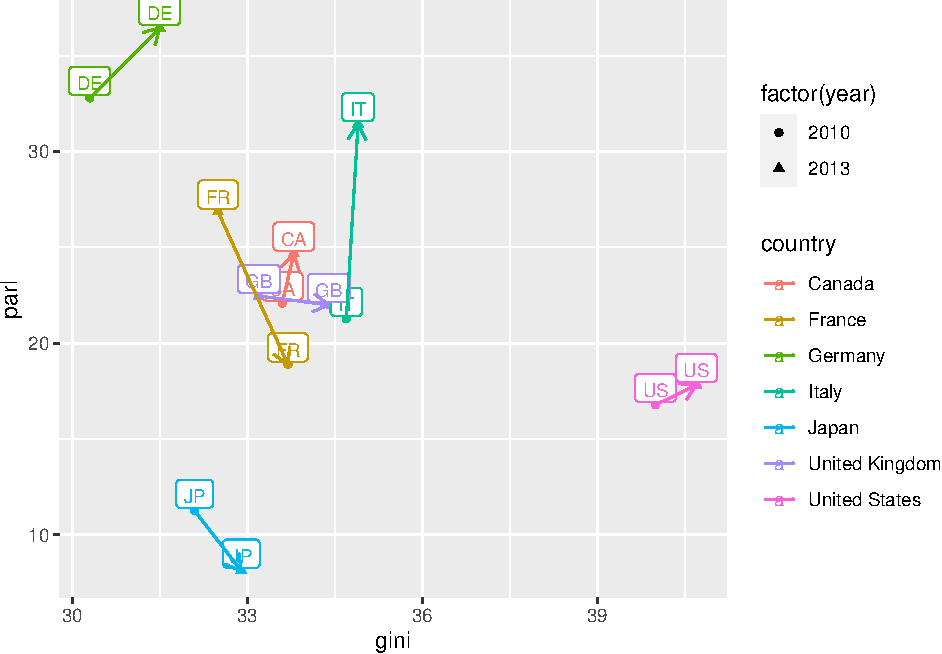
\includegraphics{le-map_revised_files/figure-latex/unnamed-chunk-16-1.pdf}

\hypertarget{review}{%
\subsection{Review}\label{review}}

\begin{itemize}
\tightlist
\item
  There seems to be missing data, i.e., the regions colored gray. Please
  check the map data as well.
\end{itemize}

\hypertarget{gini-map-of-vietnam-part-ii}{%
\section{Gini Map of Vietnam, Part
II}\label{gini-map-of-vietnam-part-ii}}

\hypertarget{get-map-data-of-vietnam-from-gadm}{%
\subsection{Get map data of Vietnam from
GADM}\label{get-map-data-of-vietnam-from-gadm}}

\begin{Shaded}
\begin{Highlighting}[]
\FunctionTok{library}\NormalTok{(geodata)}
\end{Highlighting}
\end{Shaded}

\begin{verbatim}
## Loading required package: terra
\end{verbatim}

\begin{verbatim}
## terra 1.7.28
\end{verbatim}

\begin{verbatim}
## 
## Attaching package: 'terra'
\end{verbatim}

\begin{verbatim}
## The following object is masked from 'package:tidyr':
## 
##     extract
\end{verbatim}

\begin{Shaded}
\begin{Highlighting}[]
\NormalTok{map\_vietnam0 }\OtherTok{\textless{}{-}} \FunctionTok{gadm}\NormalTok{(}\AttributeTok{country=}\StringTok{"VNM"}\NormalTok{, }\AttributeTok{level=}\DecValTok{1}\NormalTok{, }\AttributeTok{path=}\FunctionTok{tempdir}\NormalTok{())}
\FunctionTok{class}\NormalTok{(map\_vietnam0)}
\end{Highlighting}
\end{Shaded}

\begin{verbatim}
## [1] "SpatVector"
## attr(,"package")
## [1] "terra"
\end{verbatim}

\begin{Shaded}
\begin{Highlighting}[]
\FunctionTok{plot}\NormalTok{(map\_vietnam0)}
\end{Highlighting}
\end{Shaded}

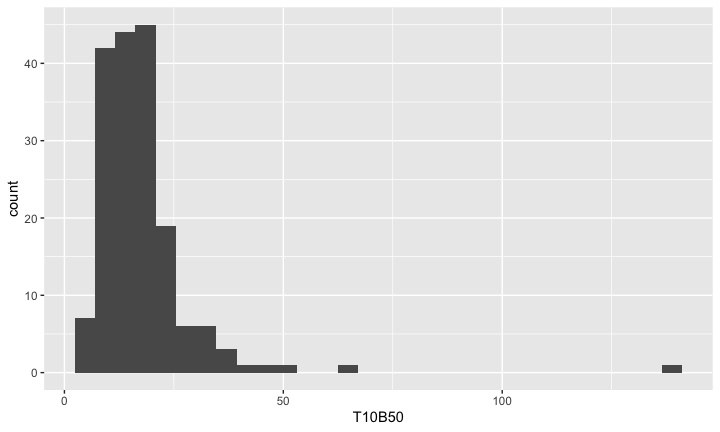
\includegraphics{le-map_revised_files/figure-latex/unnamed-chunk-18-1.pdf}

\begin{Shaded}
\begin{Highlighting}[]
\NormalTok{map\_vietnam0}
\end{Highlighting}
\end{Shaded}

\begin{verbatim}
##  class       : SpatVector 
##  geometry    : polygons 
##  dimensions  : 63, 11  (geometries, attributes)
##  extent      : 102.1446, 109.4692, 8.381355, 23.39269  (xmin, xmax, ymin, ymax)
##  coord. ref. : lon/lat WGS 84 (EPSG:4326) 
##  names       :   GID_1 GID_0 COUNTRY            NAME_1         VARNAME_1
##  type        :   <chr> <chr>   <chr>             <chr>             <chr>
##  values      : VNM.1_1   VNM Vietnam          An Giang          An Giang
##                VNM.7_1   VNM Vietnam Bà Rịa - Vũng Tàu Ba Ria - Vung Tau
##                VNM.3_1   VNM Vietnam         Bắc Giang         Bac Giang
##  NL_NAME_1 TYPE_1 ENGTYPE_1  CC_1 HASC_1 ISO_1
##      <chr>  <chr>     <chr> <chr>  <chr> <chr>
##         NA   Tỉnh  Province    NA  VN.AG VN-44
##         NA   Tỉnh  Province    NA  VN.BV    NA
##         NA   Tỉnh  Province    NA  VN.BG    NA
\end{verbatim}

\begin{Shaded}
\begin{Highlighting}[]
\NormalTok{map\_vietnam00 }\OtherTok{\textless{}{-}} \FunctionTok{st\_as\_sf}\NormalTok{(map\_vietnam0, }\AttributeTok{row.names=}\ConstantTok{NULL}\NormalTok{, }\AttributeTok{optional=}\ConstantTok{FALSE}\NormalTok{, }\AttributeTok{geom=}\ConstantTok{NULL}\NormalTok{)}
\NormalTok{map\_vietnam00}
\end{Highlighting}
\end{Shaded}

\begin{verbatim}
## Simple feature collection with 63 features and 11 fields
## Geometry type: GEOMETRY
## Dimension:     XY
## Bounding box:  xmin: 102.1446 ymin: 8.381355 xmax: 109.4692 ymax: 23.39269
## Geodetic CRS:  WGS 84
## First 10 features:
##       GID_1 GID_0 COUNTRY            NAME_1         VARNAME_1 NL_NAME_1 TYPE_1
## 1   VNM.1_1   VNM Vietnam          An Giang          An Giang      <NA>   Tỉnh
## 2   VNM.7_1   VNM Vietnam Bà Rịa - Vũng Tàu Ba Ria - Vung Tau      <NA>   Tỉnh
## 3   VNM.3_1   VNM Vietnam         Bắc Giang         Bac Giang      <NA>   Tỉnh
## 4   VNM.4_1   VNM Vietnam           Bắc Kạn           Bac Kan      <NA>   Tỉnh
## 5   VNM.2_1   VNM Vietnam          Bạc Liêu          Bac Lieu      <NA>   Tỉnh
## 6   VNM.5_1   VNM Vietnam          Bắc Ninh          Bac Ninh      <NA>   Tỉnh
## 7   VNM.6_1   VNM Vietnam           Bến Tre           Ben Tre      <NA>   Tỉnh
## 8   VNM.8_1   VNM Vietnam         Bình Định         Binh Dinh      <NA>   Tỉnh
## 9   VNM.9_1   VNM Vietnam        Bình Dương        Binh Duong      <NA>   Tỉnh
## 10 VNM.10_1   VNM Vietnam        Bình Phước        Binh Phuoc      <NA>   Tỉnh
##    ENGTYPE_1 CC_1 HASC_1 ISO_1                       geometry
## 1   Province <NA>  VN.AG VN-44 POLYGON ((105.5486 10.42948...
## 2   Province <NA>  VN.BV  <NA> MULTIPOLYGON (((107.0901 10...
## 3   Province <NA>  VN.BG  <NA> POLYGON ((106.2838 21.13225...
## 4   Province <NA>  VN.BK  <NA> POLYGON ((105.8724 21.85575...
## 5   Province <NA>  VN.BL  <NA> POLYGON ((105.4244 9.021305...
## 6   Province <NA>  VN.BN  <NA> POLYGON ((106.1306 20.99494...
## 7   Province <NA>  VN.BR  <NA> POLYGON ((106.719 10.03367,...
## 8   Province <NA>  VN.BD  <NA> MULTIPOLYGON (((109.3704 13...
## 9   Province <NA>  VN.BI  <NA> POLYGON ((106.7613 10.87455...
## 10  Province <NA>  VN.BP  <NA> POLYGON ((106.8665 11.31349...
\end{verbatim}

\begin{Shaded}
\begin{Highlighting}[]
\NormalTok{vietnam\_gini\_map00 }\OtherTok{\textless{}{-}}\NormalTok{ map\_vietnam00 }\SpecialCharTok{\%\textgreater{}\%} \FunctionTok{left\_join}\NormalTok{(gini\_vietnam, }\AttributeTok{by =} \FunctionTok{c}\NormalTok{(}\StringTok{"VARNAME\_1"} \OtherTok{=} \StringTok{"province"}\NormalTok{))}
\NormalTok{vietnam\_gini\_map00}
\end{Highlighting}
\end{Shaded}

\begin{verbatim}
## Simple feature collection with 63 features and 26 fields
## Geometry type: GEOMETRY
## Dimension:     XY
## Bounding box:  xmin: 102.1446 ymin: 8.381355 xmax: 109.4692 ymax: 23.39269
## Geodetic CRS:  WGS 84
## First 10 features:
##       GID_1 GID_0 COUNTRY            NAME_1         VARNAME_1 NL_NAME_1 TYPE_1
## 1   VNM.1_1   VNM Vietnam          An Giang          An Giang      <NA>   Tỉnh
## 2   VNM.7_1   VNM Vietnam Bà Rịa - Vũng Tàu Ba Ria - Vung Tau      <NA>   Tỉnh
## 3   VNM.3_1   VNM Vietnam         Bắc Giang         Bac Giang      <NA>   Tỉnh
## 4   VNM.4_1   VNM Vietnam           Bắc Kạn           Bac Kan      <NA>   Tỉnh
## 5   VNM.2_1   VNM Vietnam          Bạc Liêu          Bac Lieu      <NA>   Tỉnh
## 6   VNM.5_1   VNM Vietnam          Bắc Ninh          Bac Ninh      <NA>   Tỉnh
## 7   VNM.6_1   VNM Vietnam           Bến Tre           Ben Tre      <NA>   Tỉnh
## 8   VNM.8_1   VNM Vietnam         Bình Định         Binh Dinh      <NA>   Tỉnh
## 9   VNM.9_1   VNM Vietnam        Bình Dương        Binh Duong      <NA>   Tỉnh
## 10 VNM.10_1   VNM Vietnam        Bình Phước        Binh Phuoc      <NA>   Tỉnh
##    ENGTYPE_1 CC_1 HASC_1 ISO_1 id                              sub region
## 1   Province <NA>  VN.AG VN-44 57                      Mekong River Delta
## 2   Province <NA>  VN.BV  <NA> NA                                    <NA>
## 3   Province <NA>  VN.BG  <NA> 20    Northern midlands and mountain areas
## 4   Province <NA>  VN.BK  <NA> 14    Northern midlands and mountain areas
## 5   Province <NA>  VN.BL  <NA> 62                      Mekong River Delta
## 6   Province <NA>  VN.BN  <NA>  3                         Red River Delta
## 7   Province <NA>  VN.BR  <NA> 53                      Mekong River Delta
## 8   Province <NA>  VN.BD  <NA> 35 North Central and Central coastal areas
## 9   Province <NA>  VN.BI  <NA> 47                              South East
## 10  Province <NA>  VN.BP  <NA> 45                              South East
##       gini     icgap    top20 GDP 2021 (Billion VND) GDPPC (Thoudsand VND)
## 1  0.33112  6.411043 42.89568                92237.9              48304.49
## 2       NA        NA       NA                     NA                    NA
## 3  0.28528  4.836797 39.85996               129836.7              69237.38
## 4  0.42468 11.378723 50.28679                13531.4              41800.99
## 5  0.21500  3.367358 33.85097                53016.4              57720.00
## 6  0.28756  4.984416 38.98663               227614.6             155586.04
## 7  0.34644  6.582817 44.09636                55964.2              43192.25
## 8  0.35220  7.840459 43.28478                95311.4              63190.44
## 9  0.23180  3.457135 34.74600               408860.0             157448.23
## 10 0.29640  5.214929 40.43912                77838.4              75992.54
##    Investment   emp   lit edu     pop poprate    ubrate General average income
## 1    13186.19 46.28 91.28 7.0 1909.51    0.26 33.831893                   3406
## 2          NA    NA    NA  NA      NA      NA        NA                     NA
## 3    62895.00 50.41 98.20 5.8 1875.24    1.81 18.219535                   3966
## 4     3720.44 43.27 93.49 8.1  323.71    2.26 22.585030                   2125
## 5    31860.78 51.25 94.48 4.6  918.51    0.55 27.755822                   3642
## 6    58219.00 51.02 98.35 9.7 1462.95    3.04 36.648553                   4917
## 7    20099.00 58.74 94.46 4.2 1295.70    0.26  9.899668                   3367
## 8    42366.00 53.97 96.35 8.3 1508.32    1.36 41.159038                   3469
## 9   123370.26 62.40 97.30 6.6 2596.79    0.63 84.322567                   7123
## 10   25707.59 56.95 93.44 5.4 1024.29    1.30 24.166984                   4002
##                          geometry
## 1  POLYGON ((105.5486 10.42948...
## 2  MULTIPOLYGON (((107.0901 10...
## 3  POLYGON ((106.2838 21.13225...
## 4  POLYGON ((105.8724 21.85575...
## 5  POLYGON ((105.4244 9.021305...
## 6  POLYGON ((106.1306 20.99494...
## 7  POLYGON ((106.719 10.03367,...
## 8  MULTIPOLYGON (((109.3704 13...
## 9  POLYGON ((106.7613 10.87455...
## 10 POLYGON ((106.8665 11.31349...
\end{verbatim}

\includegraphics{le-map_revised_files/figure-latex/unnamed-chunk-22-1.pdf}

\hypertarget{gini-map-of-vietnam-part-iii---your-code}{%
\section{Gini Map of Vietnam, Part III - Your
Code}\label{gini-map-of-vietnam-part-iii---your-code}}

\begin{Shaded}
\begin{Highlighting}[]
\NormalTok{mapvn0 }\OtherTok{\textless{}{-}} \FunctionTok{gadm}\NormalTok{(}\AttributeTok{country =} \StringTok{"VNM"}\NormalTok{, }\AttributeTok{path =} \FunctionTok{tempdir}\NormalTok{(), }\AttributeTok{level =} \DecValTok{1}\NormalTok{)}
\FunctionTok{plot}\NormalTok{(mapvn0)}
\end{Highlighting}
\end{Shaded}

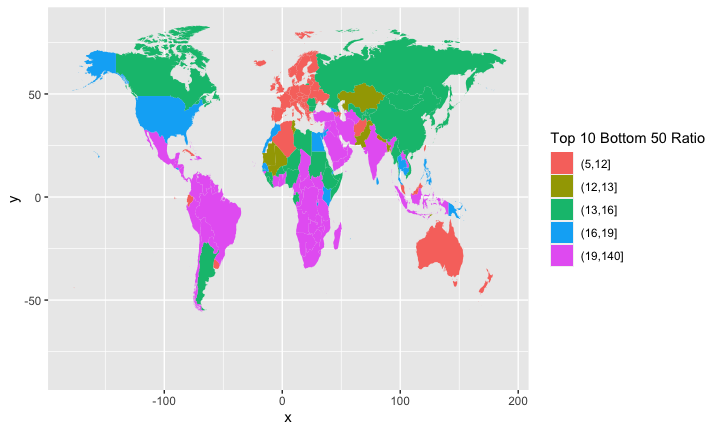
\includegraphics{le-map_revised_files/figure-latex/unnamed-chunk-23-1.pdf}

\begin{Shaded}
\begin{Highlighting}[]
\NormalTok{mapvn }\OtherTok{\textless{}{-}} \FunctionTok{st\_as\_sf}\NormalTok{(mapvn0) }\CommentTok{\#the data was already saved as data frames after this command}
\end{Highlighting}
\end{Shaded}

\begin{Shaded}
\begin{Highlighting}[]
\FunctionTok{head}\NormalTok{(mapvn)}
\end{Highlighting}
\end{Shaded}

\begin{verbatim}
## Simple feature collection with 6 features and 11 fields
## Geometry type: GEOMETRY
## Dimension:     XY
## Bounding box:  xmin: 104.7784 ymin: 9.01717 xmax: 107.5714 ymax: 22.74153
## Geodetic CRS:  WGS 84
##     GID_1 GID_0 COUNTRY            NAME_1         VARNAME_1 NL_NAME_1 TYPE_1
## 1 VNM.1_1   VNM Vietnam          An Giang          An Giang      <NA>   Tỉnh
## 2 VNM.7_1   VNM Vietnam Bà Rịa - Vũng Tàu Ba Ria - Vung Tau      <NA>   Tỉnh
## 3 VNM.3_1   VNM Vietnam         Bắc Giang         Bac Giang      <NA>   Tỉnh
## 4 VNM.4_1   VNM Vietnam           Bắc Kạn           Bac Kan      <NA>   Tỉnh
## 5 VNM.2_1   VNM Vietnam          Bạc Liêu          Bac Lieu      <NA>   Tỉnh
## 6 VNM.5_1   VNM Vietnam          Bắc Ninh          Bac Ninh      <NA>   Tỉnh
##   ENGTYPE_1 CC_1 HASC_1 ISO_1                       geometry
## 1  Province <NA>  VN.AG VN-44 POLYGON ((105.5486 10.42948...
## 2  Province <NA>  VN.BV  <NA> MULTIPOLYGON (((107.0901 10...
## 3  Province <NA>  VN.BG  <NA> POLYGON ((106.2838 21.13225...
## 4  Province <NA>  VN.BK  <NA> POLYGON ((105.8724 21.85575...
## 5  Province <NA>  VN.BL  <NA> POLYGON ((105.4244 9.021305...
## 6  Province <NA>  VN.BN  <NA> POLYGON ((106.1306 20.99494...
\end{verbatim}

\begin{Shaded}
\begin{Highlighting}[]
\FunctionTok{write.csv}\NormalTok{(mapvn,}\StringTok{"mapvn.csv"}\NormalTok{,}\AttributeTok{row.names=}\ConstantTok{TRUE}\NormalTok{)}
\FunctionTok{names}\NormalTok{(mapvn)}
\end{Highlighting}
\end{Shaded}

\begin{verbatim}
##  [1] "GID_1"     "GID_0"     "COUNTRY"   "NAME_1"    "VARNAME_1" "NL_NAME_1"
##  [7] "TYPE_1"    "ENGTYPE_1" "CC_1"      "HASC_1"    "ISO_1"     "geometry"
\end{verbatim}

\begin{Shaded}
\begin{Highlighting}[]
\NormalTok{mapvn\_gini }\OtherTok{\textless{}{-}}\NormalTok{ mapvn }\SpecialCharTok{\%\textgreater{}\%} \FunctionTok{left\_join}\NormalTok{(gini\_vietnam, }\AttributeTok{by =} \FunctionTok{c}\NormalTok{(}\StringTok{"VARNAME\_1"} \OtherTok{=} \StringTok{"province"}\NormalTok{))}
\NormalTok{mapvn\_gini}
\end{Highlighting}
\end{Shaded}

\begin{verbatim}
## Simple feature collection with 63 features and 26 fields
## Geometry type: GEOMETRY
## Dimension:     XY
## Bounding box:  xmin: 102.1446 ymin: 8.381355 xmax: 109.4692 ymax: 23.39269
## Geodetic CRS:  WGS 84
## First 10 features:
##       GID_1 GID_0 COUNTRY            NAME_1         VARNAME_1 NL_NAME_1 TYPE_1
## 1   VNM.1_1   VNM Vietnam          An Giang          An Giang      <NA>   Tỉnh
## 2   VNM.7_1   VNM Vietnam Bà Rịa - Vũng Tàu Ba Ria - Vung Tau      <NA>   Tỉnh
## 3   VNM.3_1   VNM Vietnam         Bắc Giang         Bac Giang      <NA>   Tỉnh
## 4   VNM.4_1   VNM Vietnam           Bắc Kạn           Bac Kan      <NA>   Tỉnh
## 5   VNM.2_1   VNM Vietnam          Bạc Liêu          Bac Lieu      <NA>   Tỉnh
## 6   VNM.5_1   VNM Vietnam          Bắc Ninh          Bac Ninh      <NA>   Tỉnh
## 7   VNM.6_1   VNM Vietnam           Bến Tre           Ben Tre      <NA>   Tỉnh
## 8   VNM.8_1   VNM Vietnam         Bình Định         Binh Dinh      <NA>   Tỉnh
## 9   VNM.9_1   VNM Vietnam        Bình Dương        Binh Duong      <NA>   Tỉnh
## 10 VNM.10_1   VNM Vietnam        Bình Phước        Binh Phuoc      <NA>   Tỉnh
##    ENGTYPE_1 CC_1 HASC_1 ISO_1 id                              sub region
## 1   Province <NA>  VN.AG VN-44 57                      Mekong River Delta
## 2   Province <NA>  VN.BV  <NA> NA                                    <NA>
## 3   Province <NA>  VN.BG  <NA> 20    Northern midlands and mountain areas
## 4   Province <NA>  VN.BK  <NA> 14    Northern midlands and mountain areas
## 5   Province <NA>  VN.BL  <NA> 62                      Mekong River Delta
## 6   Province <NA>  VN.BN  <NA>  3                         Red River Delta
## 7   Province <NA>  VN.BR  <NA> 53                      Mekong River Delta
## 8   Province <NA>  VN.BD  <NA> 35 North Central and Central coastal areas
## 9   Province <NA>  VN.BI  <NA> 47                              South East
## 10  Province <NA>  VN.BP  <NA> 45                              South East
##       gini     icgap    top20 GDP 2021 (Billion VND) GDPPC (Thoudsand VND)
## 1  0.33112  6.411043 42.89568                92237.9              48304.49
## 2       NA        NA       NA                     NA                    NA
## 3  0.28528  4.836797 39.85996               129836.7              69237.38
## 4  0.42468 11.378723 50.28679                13531.4              41800.99
## 5  0.21500  3.367358 33.85097                53016.4              57720.00
## 6  0.28756  4.984416 38.98663               227614.6             155586.04
## 7  0.34644  6.582817 44.09636                55964.2              43192.25
## 8  0.35220  7.840459 43.28478                95311.4              63190.44
## 9  0.23180  3.457135 34.74600               408860.0             157448.23
## 10 0.29640  5.214929 40.43912                77838.4              75992.54
##    Investment   emp   lit edu     pop poprate    ubrate General average income
## 1    13186.19 46.28 91.28 7.0 1909.51    0.26 33.831893                   3406
## 2          NA    NA    NA  NA      NA      NA        NA                     NA
## 3    62895.00 50.41 98.20 5.8 1875.24    1.81 18.219535                   3966
## 4     3720.44 43.27 93.49 8.1  323.71    2.26 22.585030                   2125
## 5    31860.78 51.25 94.48 4.6  918.51    0.55 27.755822                   3642
## 6    58219.00 51.02 98.35 9.7 1462.95    3.04 36.648553                   4917
## 7    20099.00 58.74 94.46 4.2 1295.70    0.26  9.899668                   3367
## 8    42366.00 53.97 96.35 8.3 1508.32    1.36 41.159038                   3469
## 9   123370.26 62.40 97.30 6.6 2596.79    0.63 84.322567                   7123
## 10   25707.59 56.95 93.44 5.4 1024.29    1.30 24.166984                   4002
##                          geometry
## 1  POLYGON ((105.5486 10.42948...
## 2  MULTIPOLYGON (((107.0901 10...
## 3  POLYGON ((106.2838 21.13225...
## 4  POLYGON ((105.8724 21.85575...
## 5  POLYGON ((105.4244 9.021305...
## 6  POLYGON ((106.1306 20.99494...
## 7  POLYGON ((106.719 10.03367,...
## 8  MULTIPOLYGON (((109.3704 13...
## 9  POLYGON ((106.7613 10.87455...
## 10 POLYGON ((106.8665 11.31349...
\end{verbatim}

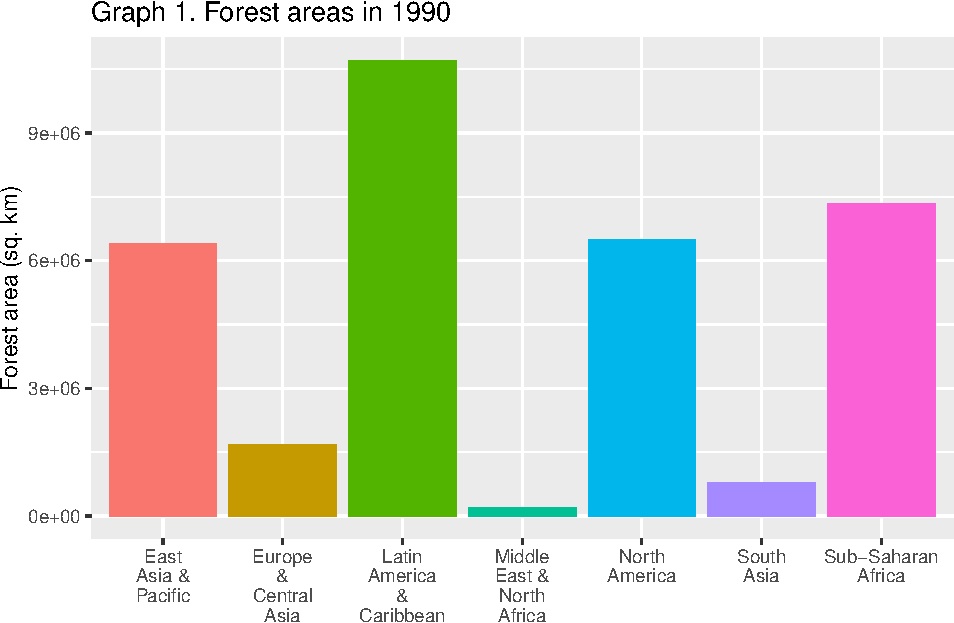
\includegraphics{le-map_revised_files/figure-latex/unnamed-chunk-28-1.pdf}

\hypertarget{review-1}{%
\subsubsection{Review}\label{review-1}}

\begin{itemize}
\tightlist
\item
  You should check the province name with those in the map data as I did
  in my first try. I leave this process to you.
\end{itemize}

\hypertarget{convert-geometry-data-into-longlat-data}{%
\subsubsection{Convert Geometry data into long/lat
data???}\label{convert-geometry-data-into-longlat-data}}

I supposed that if I can convert geometry data into long/lat data, the
map can be drawn.

I tried some solutions on the internet and the followings are one of
them, but it did not work correctly.

\hypertarget{references-same-as-yours}{%
\section{References: (same as yours)}\label{references-same-as-yours}}

\begin{enumerate}
\def\labelenumi{\arabic{enumi}.}
\tightlist
\item
  \url{https://stackoverflow.com/questions/47661354/converting-geometry-to-longitude-latitude-coordinates-in-r}
\item
  \url{https://community.rstudio.com/t/convert-geometry-column-with-lists-of-longitude-latitude-coordinates/67114/7}
\item
  \url{https://rstudio-pubs-static.s3.amazonaws.com/647153_88833beacf2c4107ad76bc3bc7bc8b9d.html}
\item
  \url{https://rdrr.io/cran/terra/man/as.data.frame.html} This one:
  \url{https://stackoverflow.com/questions/73825468/converting-spatvector-objects-to-data-frames-for-use-in-ggplot2}
\end{enumerate}

\end{document}
